\chapter{"user" szintű felhasználói felületek, és azok működése}
\label{chap:fejezet5}

A fogászati rendelő alkalmazás számos felülettel rendelkezik.

\section{A bejelentkezés és a regisztráció működése}

Az alkalmazásomban a regisztráció és bejelentkezés funkciók a Django beépített autentikációs rendszerére épülnek, amely lehetővé teszi a felhasználók kezelését, hitelesítését és jogosultságainak kezelését. Ez a funkció azért hasznos egy fejlesztőnek, mert ezáltal nem kell ezeket implementálnia minden új projektjébe.

\subsection{Az alkalmazás autentikációra használt metódusai:}

\begin{itemize}
	\item "authenticate": Ez a metódus ellenőrzi a felhasználó hitelesítő adatait (email és jelszó). Az EmailBackend osztály implementálja az "authentication.py" fájlban, és az email cím alapján keresi meg a felhasználót.
	\item "auth\_login": Bejelentkezteti a felhasználót, és a munkamenethez társítja. A Django beépített metódusa.
	\item "check\_password": Ellenőrzi, hogy a megadott jelszó megegyezik-e a titkosított jelszóval. A Django beépített metódusa.
	\item "set\_password": Beállítja az adott felhasználónak a jelszavát, és hashelt formában elmenti az adatbázisba. A Django beépített metódusa.
	\item "get\_user": Lekéri a felhasználót az azonosítója alapján. A Django beépített metódusa.
\end{itemize}

\begin{figure}[!htbp]
	\caption{Az "authentication.py"}
	\label{fig:authentication}
	\centering
	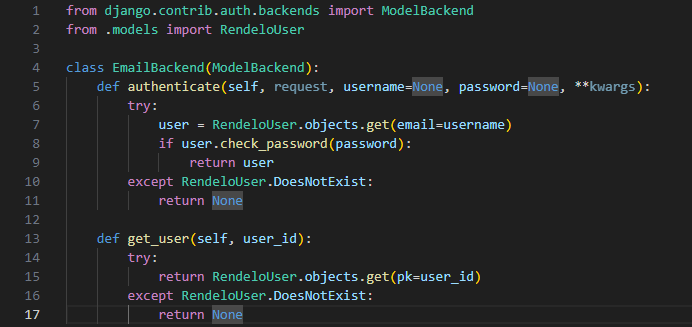
\includegraphics[width=1.0\textwidth]{authentication_py.png}
\end{figure}

\subsection{Regisztráció}

A regisztráció során a felhasználó a "register.html" fájlban megvalósított oldalon létrehozhat egy új fiókot, amelyet a rendszer a "RendeloUser" model-ben tárol. A regisztrációs folyamat a következőképpen működik:

\begin{enumerate}
	\item Amikor a felhasználó megnyitja a regisztrációs oldalt, a "register\_view" nézet megjeleníti a regisztrációs űrlapot. Az űrlap két részből áll: a "RegistrationForm" a felhasználói fiók alapvető adatait (például felhasználónév, email cím, jelszó) kezeli, míg a "PatientForm" a páciens adatait (például név, születési dátum) tartalmazza.
	\item Az űrlap elküldése után a "register\_view" nézet ellenőrzi az űrlapok érvényességét. Ha az adatok helyesek, a "RegistrationForm" "save" metódusa létrehoz egy új RendeloUser példányt, amely a felhasználói fiókot reprezentálja. A jelszó titkosítva kerül tárolásra a "set\_password" metódus segítségével, ami az "AbstractUser" metódusa, amiből a "RendeloUser" osztály származik.
	\item A "PatientForm" létrehoz egy új Patient példányt, amely a páciens adatait tárolja. A "register\_view" nézet pedig beállítja a Patient $id$ adattagjának az értékét az újonnan létrehozott RendeloUser $id$ adattagjának az értékére, hogy a Patient példány azonosítója megegyezzen a RendeloUser példány azonosítójával, így a két objektum összekapcsolódhasson.
	\item A regisztráció sikeres befejezése után az "auth\_login" metódus automatikusan bejelentkezteti a felhasználót, és átirányítja a kezdőoldalra.
	\item A felhasználó beállított email címére egy email kerül kiküldésre, amelyben megköszöni a cég a regisztrációt. (Jelenleg egy konzolos email küldés van beállítva, csupán a demózás céljából.)
\end{enumerate}

\begin{figure}[!htbp]
	\caption{A register\_view nézet}
	\label{fig:registerview}
	\centering
	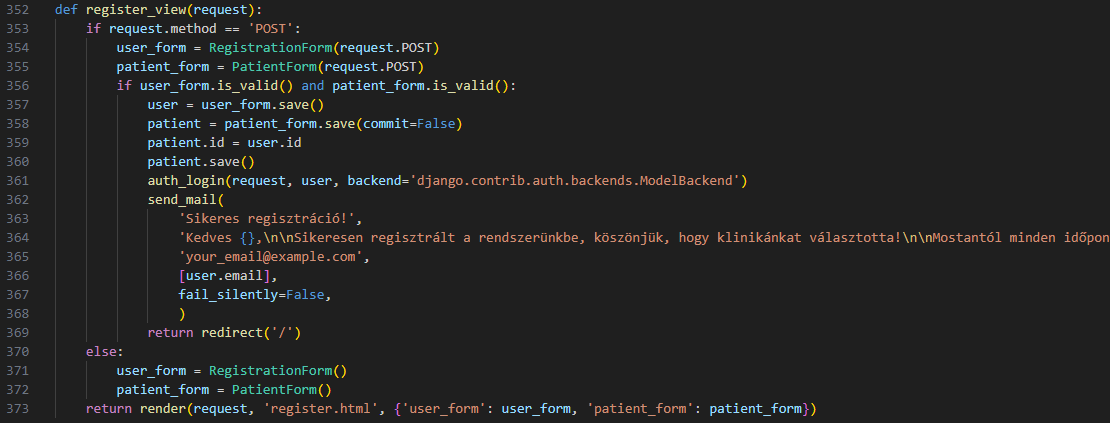
\includegraphics[width=1.0\textwidth]{register_view.png}
\end{figure}

\subsection{Bejelentkezés}

A bejelentkezés során a felhasználó a "login.html" fájlban megvalósított oldalon megadja az email címét és jelszavát, amelyek alapján a bejelentkezés történik. A folyamat a következőképpen működik:

\begin{enumerate}
	\item Amikor a felhasználó megnyitja a bejelentkezési oldalt, a "login\_view" nézet megjeleníti a bejelentkezési űrlapot. Az űrlap tartalmazza az email cím és jelszó mezőket.
	\item Az űrlap elküldése után a "login\_view" nézet az authentication.py "EmailBackend" osztályának "authenticate" metódusát hívja meg, amely az email cím és jelszó páros érvényességét ellenőrzi. Az "authenticate" metódus a "RendeloUser" modellben keresi meg a felhasználót az email cím alapján, majd a "check\_password" metódussal ellenőrzi a jelszót.
	\item Ha a hitelesítés sikeres, az "auth\_login" metódus bejelentkezteti a felhasználót, és a munkamenethez társítja. Ezután a felhasználó átirányításra kerül a kezdőoldalra.
	\item Ha a hitelesítés sikertelen (például helytelen email cím vagy jelszó miatt), a rendszer hibaüzenetet jelenít meg a felhasználónak.
\end{enumerate}

\section{A kezdőoldal}

Az összes szintű felhasználó bejelentkezés után a kezdőoldalon találja magát, amit a kezdooldal.html fájlban valósítottam meg. Az oldalon található a base.html elemein kívül egy marketing leírás a rendelőről, ami statikusan az oldalra van írva, nem lehet változtatni, csak a HTML kódban.
A leírás után pedig egy táblázat a rendelőben lehetséges kezelésekről, és azok árairól. A táblázat fejléce után Django sablon nyelven következik egy for ciklus, ami végigmegy az összes "Treatment" példányon az adatbázisban, és mindegyiknek a nevét, és az árát kiírja egy külön sorba. A Django Template fájlok az adatbázis objektumait a views.py egyik függvényétől kapják meg az 1.7. ábrán látható módon.

\begin{figure}[!htbp]
	\caption{A kezdőoldal views.py-ban található megjelenítési függvénye}
	\label{fig:kezdooldal}
	\centering
	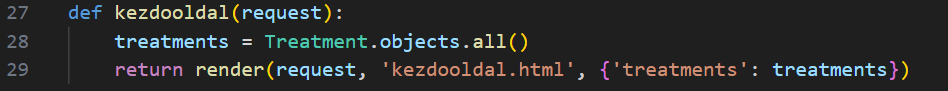
\includegraphics[width=1.0\textwidth]{kezdooldal_view.png}
\end{figure}

\section{Az időpontfoglalás}

Az időpontfoglalás oldal az egyik legösszetettebb része az alkalmazásnak. A foglalási folyamat során a felhasználó kiválasztja az orvost, a kezelést, a dátumot és az időpontot, majd a fizetési módot, ezzel elindítva az időpontfoglalás teljes folyamatát. A views.py fájlban definiált "idopontfoglalas" függvény koordinálja a folyamatot.

\subsection{Az időpontfoglalás lépései}
\begin{enumerate}
	\item Orvos kiválasztása:
	\begin{itemize}
		\item Interakció: A felhasználó az oldal tetején megjelenített orvosok listájából választ.
		\item Kód: JavaScript eseménykezelő aktiválódik, amely beállítja a "selected\_doctor" mező értékét a kiválasztott orvos azonosítójára, majd meghívja az "updateAvailableSlots()" függvényt.
	\end{itemize}
	\item Kezelés kiválasztása:
	\begin{itemize}
		\item Interakció: A felhasználó a legördülő menüből választja ki a kívánt kezelést.
		\item Kód: A kezelési opció módosítása szintén az "updateAvailableSlots()" függvényt indítja el, frissítve a kezeléshez tartozó időpontokat.
	\end{itemize}
	\item Dátum kiválasztása:
	\begin{itemize}
		\item Interakció: A felhasználó a naptármezőből választja ki a foglalni kívánt napot.
		\item Kód: A dátumválasztás után a JavaScript lekéri az adott napra vonatkozó szabad időpontokat az API végpontból, majd megjeleníti azokat.
	\end{itemize}
	\item Időpont kiválasztása:
	\begin{itemize}
		\item Interakció: A megjelenített időpontgombok közül a felhasználó kiválaszt egyet, vagy rákattint a "legközelebbi időpont" gombra.
		\item Kód: A kiválasztáskor a JavaScript beállítja az "appointment\_datetime" mező értékét (dátum és idő kombináció), illetve vizuálisan kiemeli a kiválasztott időpontot.
	\end{itemize}
	
	 Itt kihívásként említeném a felhasználó számára megjelenített elérhető időpontok megjelenítését. Azt kellett megoldanom, hogy ne csúszhassanak egymásba az időpontok. Tehát például ha le van foglalva valamilyen kezelésre egy időpont az adott dátumon 11:00-ra, akkor ne jeleníthessen meg a felhasználónak 10:45-re szabad időpontot, amikor egy 35 perc hosszúságú kezelést választott ki. Ezt az 5.4. ábrán látható metódussal oldottam meg, amit az "idopontfoglalas.html" JS kódja hív meg. A metódus először is 15-tel osztható számra kerekíti a kiválasztott kezelés hosszát felfelé, (például egy 50 perces kezelés hosszát 60 percesre kerekít), majd a HTML oldalon lévő JS kód által megjelenített időpontokat szűri. A get\_available\_slots metódus biztosítja, hogy csak azok az időpontok jelenjenek meg a felhasználónak, amelyek nem ütköznek más foglalásokkal. Ehhez a metódus minden egyes időintervallumot ellenőriz, hogy az adott időpontban és az azt követő időtartamban (a kezelés hossza alapján) ne legyen másik foglalás. A metódus figyelembe veszi az orvos munkaidejét is, így csak az orvos által megadott munkaidőn belüli időpontokat jeleníti meg. Az eredmény egy JSON válasz, amely tartalmazza az elérhető időpontokat és azok elérhetőségét. Ez a válasz a frontend JavaScript kódjában kerül feldolgozásra, amely a felhasználó számára vizuálisan is megjeleníti a szabad időpontokat.
	 
	  \begin{figure}[!htbp]
	 	\caption{A get\_avaliable\_slots metódus implementációja a views.py-ban}
	 	\label{fig:getavaliableslots}
	 	\centering
	 	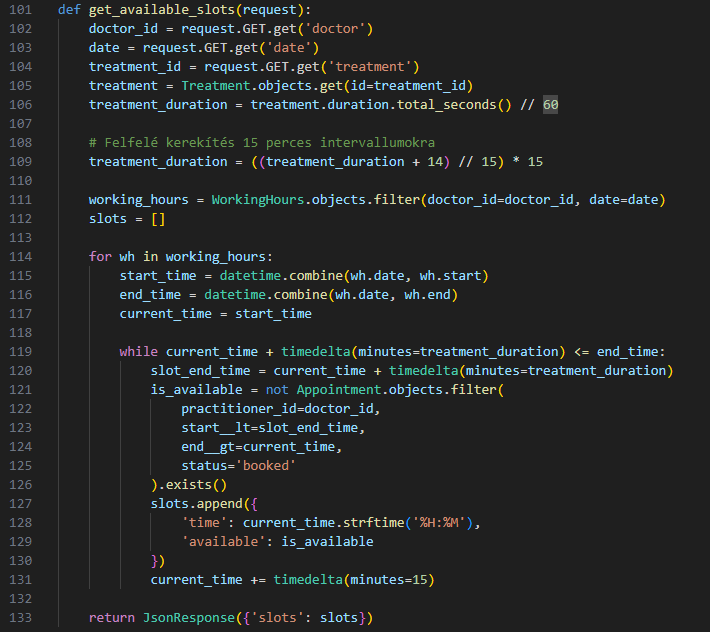
\includegraphics[width=1.0\textwidth]{get_avaliable_slots.png}
	 \end{figure}
	 
	 	\item Fizetési mód kiválasztása:
	 \begin{itemize}
	 	\item Interakció: A fizetési módok közül a felhasználó egyet választ (pl. online fizetés – PayPal vagy bankkártya, illetve helyszíni fizetés).
	 	\item Kód: A JavaScript eseménykezelő beállítja a "payment\_method" mezőt, amely később a Django backendben a foglalás véglegesítéséhez és a fizetési folyamat elindításához szükséges.
	 \end{itemize}
	 \item Foglalás véglegesítése:
	 \begin{itemize}
	 	\item Interakció: A felhasználó a „Foglalás” gombra kattint, miután minden kötelező adatot megadott.
	 	\item Kód: 
	 	\begin{itemize}
	 		\item A JavaScript egy megerősítő üzenetben összegzi a kiválasztott orvos, kezelés, dátum és időpont adatait.
	 		\item Ha a felhasználó megerősít, az űrlap elküldésre kerül, és a views.py "idopontfoglalas" függvénye végrehajtja az alábbiakat:
	 		\begin{itemize}
	 			\item Ellenőrzi az időpont elérhetőségét (szabad-e az adott időintervallum).
	 			\item Lekéri az orvos munkaidejét a WorkingHours modell alapján.
	 			\item Létrehoz egy új Appointment objektumot az adatbázisban.
	 			\item Rögzíti a foglalás fizetési státuszát a PaymentStatus modell segítségével.
	 			\item Ha a felhasználó online fizetést választott, átirányítja a fizetési oldalra a tranzakció elindításához.
	 		\end{itemize}
	 	\end{itemize}
	 \end{itemize}
\end{enumerate}


\begin{itemize}
	\item "updateAvailableSlots()" JavaScript függvény:
	Lekéri a kiválasztott orvos, kezelés és dátum alapján az elérhető időpontokat az API-ból, majd megjeleníti a délelőtti és délutáni időpontokat gombok formájában.
	\item "earliestAppointmentButton" eseménykezelő:
	A „Leghamarabbi időpont kiválasztása” gomb megnyomásakor az API-tól lekéri a legkorábbi szabad időpontot, majd automatikusan beállítja a dátumot és az időpontot.
	\item Űrlap beküldése:
	A foglalási űrlap beküldése előtt a JavaScript egy megerősítő párbeszédablakban összegzi a választott opciókat, majd a felhasználó jóváhagyása esetén elküldi az űrlapot. A Django view feldolgozza a POST kérést, létrehozza az időpontfoglalást, és ha a felhasználó az online fizetést választja, akkor a fizetési oldalra irányítja át, ha pedig a fizetés a helyszínen opciót, akkor a profil oldalra.
\end{itemize}

\section{A fizetési oldal}

A fizetési oldal a "payment\_page.html" oldalon lett megvalósítva. A fizetéshez a tématervembe OTP Simple Pay fizetési rendszert írtam, viszont egy kis kutatás után a PayPal-t könnyebben beépíthetőbbnek, stabilabbnak, és jobban átláthatóbbnak találtam. Ezért inkább azt építettem be az alkalmazásba.\\
A PayPal fizetés demózásához létre kellett hoznom egy sandbox PayPal fiókot, majd az azonosítómat használva importálnom kellett az oldalra egy JavaScriptet az alábbi módon: \\ \\

\begin{lstlisting}[caption={A PayPal sandbox importja},label={lst:stringstartswith}, language={HTML}]
<script src="https://www.paypal.com/sdk/js?client-id=Abw9kvI2SEa...&currency=HUF"></script>
\end{lstlisting}

Ezután egy "div"-hez hozzá kellett adnom a "paypal-button-container" id-t, és meg kellett valósítanom a fizetési logikát, amit az alábbi módon tettem meg a HTML fájlban:
 	
\begin{lstlisting}[caption={A fizetési logika},label={lst:stringstartswith}, language={HTML}]
	<script>
	paypal.Buttons({
		createOrder: function(data, actions) {
			return actions.order.create({
				purchase_units: [{
					amount: {
						value: '1',
						currency_code: 'HUF'
					}
				}]
			});
		},
		onApprove: function(data, actions) {
			return actions.order.capture().then(function(details) {
				fetch("", {
					method: 'POST',
					headers: {
						'Content-Type': 'application/json',
						'X-CSRFToken': '{{ csrf_token }}'
					},
					body: JSON.stringify({
						orderID: data.orderID,
						status: details.status,
						orderRef: '{{ appointment.id }}'
					})
				}).then(response => {
					if (response.ok) {
						alert('A tranzakció sikeresen megtörtént: ' + details.payer.name.given_name);
						window.location.href = "";
					} else {
						alert('Hiba történt a fizetés során.');
					}
				}).catch(error => {
					console.error('Hiba történt a fizetés során:', error);
					alert('Hiba történt a fizetés során.');
				});
			});
		},
		onError: function(err) {
			console.error(err);
			alert('Hiba történt a fizetés során.');
		}
	}).render('#paypal-button-container');
	</script>
	
\end{lstlisting}
